\frame{
    \frametitle{Dijkstra}
    \framesubtitle{Single source Shortest path}
    
    \begin{itemize}[<+->]
        \item Weighted graphs
        \item Doesn't work with negative edges / cycles
        \item Works with a priority queue (\emph{min-heap})
        \item Only add to the heap if shorter than current shortest
            = a \emph{relax} operation
        \item Don't process again (cf. BFS)
    \end{itemize}
}

\frame{
    \frametitle{Dijkstra}
    \framesubtitle{Example}

    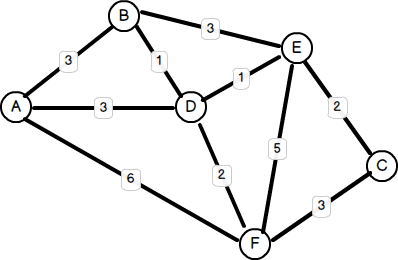
\includegraphics[width=300px]{img/weightedgraph.png}
}

\frame{
    \frametitle{Dijkstra}
    \framesubtitle{Extra remarks}
    
    \begin{itemize}[<+->]
        \item Degrades to BFS on unweighted graphs
        \item all distances from start needed $\rightarrow$ don't stop until everything is visited
        \item This is the \emph{greedy} approach
        \item $O(|E| \times \log |V|)$
        ~\\~\\~\\
        \item Why do negative weights fail?
    \end{itemize}
}
